\subsection{InteGreat}

InteGreat reinterprets bitvector-domain symbolic execution of program slices into the theory of uninterpreted functions to perform modular, nestable function summarization and lifting.
The tool provides researchers with a novel design language for automatically abstracting complex programs into mathematical equations.
In the submitted publication, InteGreat's lifting was used to determine the sensor inputs necessary to precisely destabilize the reactor pressure of a chemical plant, discover novel problems in the domain of firmware rehosting, and discover a flaw in the implemented version of a published quad-copter stabilization algorithm.

\subsubsection{Motivating Example}

To introduce InteGreat's core contributions, compare the typical operation of symbolic execution on a function in a closed-source binary firmware to InteGreat's approach.

\begin{figure}
  \centering
	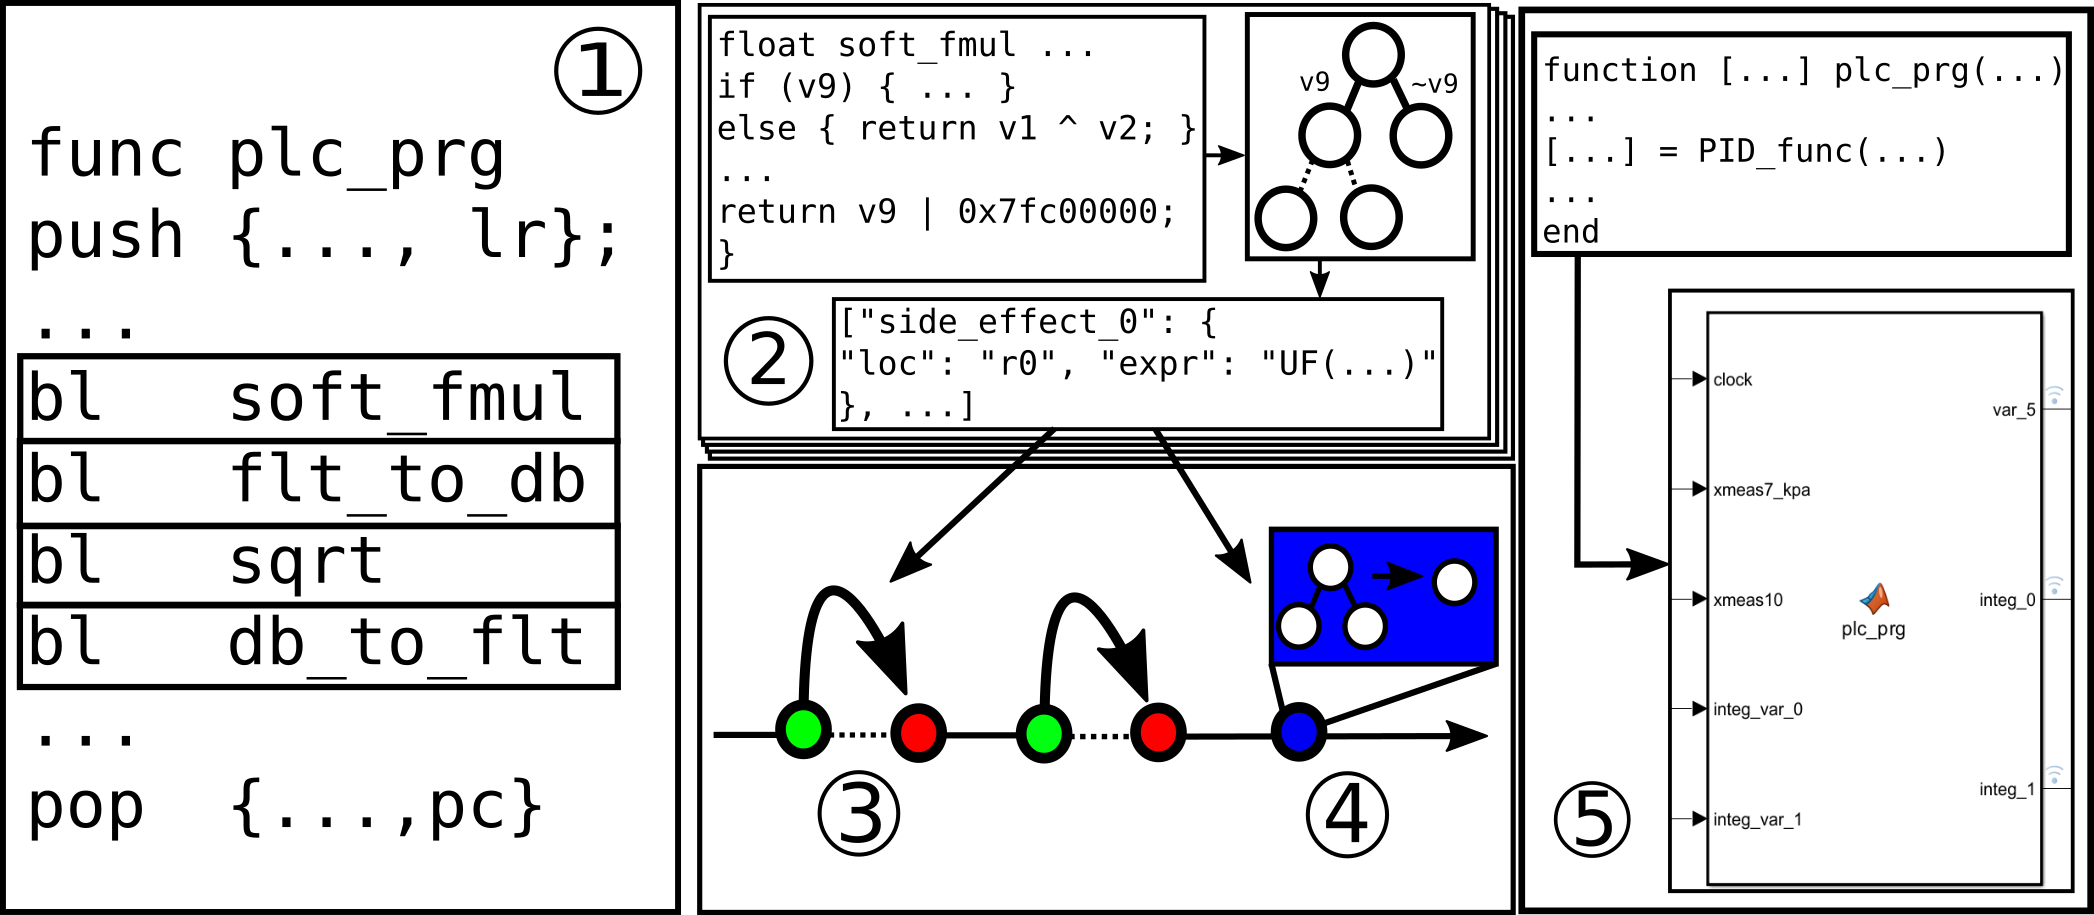
\includegraphics[width=0.7\textwidth]{integreat-example.png}
	\caption{Depiction of an example execution of InteGreat on a small program. Red/Green nodes describe abstracting a program slice. Blue stands for program slice pattern triggering higher level abstractions that stitches slices according to combination rules}
	\label{fig:integreat-example}
\end{figure}

\paragraph{Traditional Symbolic Execution.}
Traditional symbolic execution of the function presented in (1) of Fig.~\ref{fig:integreat-example} will begin by loading a symbolic state $S$ at the entry point to the function.
Between each inner call, a number of additional instructions could exist but are not depicted.
Upon reaching a child function, symbolic execution will enter this function and begin to execute it.
The symbolic executor will then proceed to accumulate all the branches, constraints, and operations in the child function.
A software floating point multiply we studied, for example, had 153 lines of pseudo-C, 116 of decompiled assembly, and 15 branches.
The symbolic executor will then exit the child function and begin executing the succeeding instruction with some $n$ possible symbolic constraint sets.
This process will continue until the end of the program is reached.
Finally, in most cases, the symbol executor will output a statement over the theory of bitvectors rather than a more abstract domain, due to the complexity of determining relevant or desired abstraction boundaries in the general case.

Complexity arises due to the lack of a general solution to the halting problem and the necessity of supporting various microarchitectural operational semantics.
A loop without an explicit guard condition within a child function may entirely sabotage symbolic execution due to \emph{state explosion}.
For example, a while-true loop may have a break condition which could fire on any of $1\dots\infty$ iterations (this is common during reads from hardware devices).
Moreover, angr~\cite{angr-1} and to our knowledge most other closed-source binary symbolic executors do not (publicly) support memory accesses to a symbolic address, as these may potentially reference the entire address space, leading to a combinatorial explosion of the possible resulting execution states. 
This issue was solved by Coppa et al.~\cite{coppa2017rethinking}, however, it was never integrated into angr~\cite{angr-2}.

\paragraph{InteGreat's Approach.} Unlike a traditional symbolic executor, InteGreat adopts a more constrained goal of lifting to continuous equations that can be loaded into a mathematical verifier or program like Matlab.
To achieve this, InteGreat provides users with a mechanism for associating program slices to symbols, and handles all the semantic ``stitching'' this entails automatically.
We assume the control flow of a given slice is completely contained within another and there may be no partial overlaps (an independence system).
A simple example of this would be the address range of a function compiled inline into the body of another function, or a call instruction itself. 
The largest slice is the program itself, and slices consist of entry and exit addresses.

First, in (1), we begin a post-order tree traversal of the program slices, descending to ``leaf'' program slices that have no inner slices. 
For simplicity, in Fig.~\ref{fig:integreat-example} we define the slices as each inner function, called to by each \emph{bl} assembly instruction.
These slices are provided to InteGreat via a JSON specification file.

Then, in (2), we generate an \emph{abstraction specification} for each given slice.
We use traditional symbolic execution to identify all the possible side-effect locations (registers, memory) of the slice for each execution path, which includes function input locations.
Note that here we have assumed the desired semantics for the slice's computation are decidable given some \emph{search strategy}.

To avoid state explosion when lifting undecidable algorithms, we leave this strategy user-configurable but provide a few sensible defaults, e.g. taking the state that generates the most complex set of constraints or the largest number of writes to memory.
However, state explosion remains a hard problem for abstract interpretation and InteGreat helps to make progress on this problem by providing a more general interface for abstracting program slices.
To cope with the problem of combinatorial pointer value explosion discussed above, we implement a version of the 2017 Coppa et al. work, representing each read or write to memory with both the value and the symbolic expression used to determine the address, discussed below.

Next, in (3), we begin the process of \emph{abstraction resolution}.
Assuming all $n$th layer slices are correctly lifted and the symbolic execution state is loaded at the beginning of each slice in the $n+1$th layer.
Symbolic execution proceeds as normal until it hits the entry point of an $n$th layer program slice $\gamma$.
In the simplest case, the symbolic execution jumps to the exit point of this slice and parameterized uninterpreted function(s) $f$ are written to the output location(s) of $\gamma$.
To parameterize $f$, the constraints and execution context at the input locations of $\gamma$ (locations are identified in (2)) are supplied as parameters to $f$.
$f$ does not have to be an uninterpreted function, but could be any (recovered) model of the child slice's semantics.
(3) continues until a higher level abstraction is triggered or the function ends (e.g. return).

(4) represents how each exit point of a program slice triggers a check for patterns specified as higher level abstractions.
Upon each pattern match, a corresponding rewrite rule is applied to the abstract symbol tree (AST) containing the symbolic constraints for the current program execution path.
This allows us, for instance, to automatically abstract out the marshalling of bitvectors to and from register pairs necessary to represent 64-bit floating point values on 32-bit architectures.

In (5) we post-process the resultant AST, linking output expressions to inputs and resolving abstractions into a model in a high-level language. 
In this paper, we target Matlab code as it provides an easy, reproducible evaluation.
At this stage, program slices are ordered by symbolic execution timestamps, and we disambiguate different pointer values passed into the same program slice using the strict equality discussed above.
Finally, we also parse side-effects into stateful variables, i.e. self-loops from output to input.
We also remove duplicate computations (AST subtrees) across multiple outputs by translating the AST into a sequence of assignments.

\subsubsection{Techniques}

InteGreat reformulates classical function summarization (introduced in Sec.~\ref{sec:func-summarization}) as \emph{nested function summarization}.
A nested function summarization is of the form $\Gamma_1, \Gamma_2 \ \ldots \ \Gamma_n$, where every $\Gamma$ is a non-empty finite set of dynamic logic formulas. 
Nested function summarizations can be reused and \emph{chained} inside of higher-level summarizations.
The decision procedure for such resolutions follows from $\Gamma$.

In order to define a nested function summarization $\Gamma$ in domain $\mathcal{D}$, we split $\Gamma$ into two sets, $\Gamma_{M}$ and $\Gamma_{S}$, representing the \emph{storage} and \emph{semantics} (expressions) of a program slice, respectively.
Given $m \in M$, $\Gamma_{M} \vdash m_{\mathcal{M}} \rightarrow m'_{\mathcal{D}}$, binding the symbols for registers and memory to the abstract domain, and $\Gamma_{S} \vdash S^{\Gamma}_{\mathcal{M}} \rightarrow S'_{\mathcal{D}}$, where $S^{\Gamma}_{\mathcal{M}} \subseteq S_{\mathcal{M}}$, a partial mapping of the semantics of the concrete domain to equivalent semantics in the abstract domain.
Partial specification allows users to avoid, for example, reproducing the microarchitecture. A given usecase may only require semantics indicated by \texttt{call} instructions.
$\Gamma$ may then be specified for new domains $\mathcal{D}, \mathcal{D}', \ldots$ by substituting $\mathcal{M}$ for the higher layer of abstraction.

We define program slices as abstraction boundaries that occur naturally in the firmware or by user definition.
Each abstraction or summarization is a decision to associate a \emph{sign} (a fresh symbolic variable) with a specific set of computations.
The set of substituted instructions, i.e. the range of summarization, must be \emph{complete}: all the program semantics which should be substituted for $f$ must be substituted ($S^{f}_{\mathcal{M}} \subseteq S^{\Gamma}_{\mathcal{M}}$).
This, for example, could require resolving the callsites indicated by dynamically assigned pointer values, something that is hard to do generally, as these values could be I/O dependent: InteGreat addresses this problem by requiring the abstraction of program slices invoking the virtual call (otherwise it will throw a fault).
Although in general this problem is also solvable using other means, e.g. symbolically executing more of the program or by using static analysis.

As a computation $S$ can have loops, we must ensure or assume that the nested function summarization $\Gamma$ is \emph{closed}, i.e. the set of operations $S^{\Gamma}_{\mathcal{M}}$ is finite.
The basic solution in cases where $S$ halts for all inputs is universal quantification or the computation of a \emph{fixed point}.
For example, let $T = \{t_{1}, t_{2}, \ldots, t_{n}\}$ be the complete set of possible traces over computations $C =c_{1}, c_{2}, \ldots, c_{n}$ in the program slice.
Then the summarization $\Gamma$ is closed if $\Gamma \vdash \bigwedge_{t \in T} \Gamma_{S} \vdash t_{\mathcal{M}} \rightarrow t'_{\mathcal{D}}$.
To allow analysis of $S^{C}_{\mathcal{M}} \notin HALT$, we use a \emph{search strategy}.
In prior work the search strategy is a bound $v$ for unrolling all loops in $S$ (Sec.~\ref{sec:func-summarization}).

\textbf{Nested Abstraction Resolution.} 
  \label{prob:abstraction-resolution}
Once the particular side-effects of a program slice are \emph{bound}, the side-effect values upon exiting the slice may be substituted with arbitrary logical operations over the program's state, similar to a standard SimProcedure in angr.
Unlike angr, InteGreat automates the nesting of procedures based upon a formula, so that more complex abstractions may be built from simpler ones.
Representing a function $f$, we construct $\Gamma \vdash S^{f}_{\mathcal{M}} \rightarrow S^{f}_{\mathcal{D}}$, but the concrete domains $\mathcal{M}$ includes abstractions previously defined by $\Gamma$ and $\mathcal{D}$ is not itself ``hard-coded'' but defined by the logical formulae used to substitute the program slices (either automatically lifted uninterpreted functions or user-specified alternative formulae for the slices' semantics).
However, any concrete implementation must restrict $\mathcal{D}$ to some finite set of supported syntaxes, e.g. QF\_UF.
InteGreat supports the same theories as Z3.


\lstdefinelanguage{json}{
    basicstyle=\footnotesize\ttfamily,
    showstringspaces=false,
    breaklines=true,
    float=tp,
    numbers=none,
    floatplacement=tbp
}

\lstset{language=json,basicstyle=\ttfamily\scriptsize}
\begin{figure}
\begin{lstlisting}
"pid": {"addrs": [<auto-populated, e.g. 0xCAFE:0xCBFE], "conf": "./pid.json"}
"derivative": {"addrs": [<auto-populated>], "conf": "./derivative.json"}
"integral": {"addrs": [<auto-populated>], "conf": "./integral.json"}
\end{lstlisting}
\vspace{5pt}
\hrule\vspace{5pt}
\begin{lstlisting}
"in":   {"i0":{"type": "float", "location": "reg", "ptr": "r0"},
         "i1":{"type": "float", "location": "reg", "ptr": "r1"}},
"out":  {"o0":{"type": "float", "location": "reg", "ptr": "r0"},
"expr": "(declare-fun F((_FloatingPoint 8 24)) Bool) ...
	(declare-funinput()(_BitVec32))(...)...
		assert(let((a!1(...(_ to_fp 8 24) i1)..."
\end{lstlisting}
% "absts"     : ['mul.json', 'integral.json', 'atan.json'],
% "out"   : {"o0": {"type": "float", "location": "stack", "ptr": "S+8"},
%            "o1": {"type": "float", "location": "mem", "ptr": "M[0x2004]+8"}},
% \begin{lstlisting}
% "slices":     [{"addr":"0xcafe:0xcaff"}],
% \end{lstlisting}
\vspace{5pt}
\hrule\vspace{5pt}
\begin{lstlisting}
"slice_expr": "f2d, muldf, trunc",
"abst_in":    {"f2d":["i0"], "muldf":["i2", "i3"]},
"abst_out":   {"trunc":["o0"]},
\end{lstlisting}
	\caption{\textbf{Top}: Example of a top-level configuration file, with symbolic execution specifications connected to a list of inference rules. \textbf{Middle}: InteGreat automatically exports this function summarization of a derivative function as a Z3 function expression with bindings to the input locations. \textbf{Bottom}: Example higher-order inference rules with references to nested program slices, used to rewrite multiplication function with type conversion to plain multiplication.} 
\label{fig:json-example}
\end{figure}

\textbf{Input.}
\label{sec:input-output}
The input to InteGreat is a firmware $F$ and a set of program slices.
Slices can take the form of a range of addresses (potentially of zero length), a type of instruction, or an expression over the names of other slices.
To avoid repeating the same abstraction in multiple places, we break this up into a set of objects, where the ``entrypoint'' object refers to the highest level of abstraction, and descendants refer to inner slices.

The top of Figure~\ref{fig:json-example} provides the list of program slices.
\emph{These slices and the JSON file hierarchy can be automatically generated from static analysis of $F$, and InteGreat provides a set of scripts covering basic use cases, e.g. abstract every child function of a given function.}
Thus, in the figure we list the addresses for the slices as ``auto-populated''.
However, we leave the decision to use auto-population scripts to the user, to avoid assumptions about $F$'s structure and the desired abstractions.

As InteGreat executes, each JSON file is populated with the inference rules $(\mathcal{I}$, $\mathcal{A})$ for lifting the program slice.
A simplified version of these outputs are given in the middle of Figure~\ref{fig:json-example}.
Importantly, it contains three parts: the input variables supplied to the inference, the side-effect locations (outputs), and the expression for the slice reinterpreted as an uninterpreted function.
Optionally, because this expression is a logical formula over the program state, the user can \emph{modify} this file after the fact and specify alternative or additional formulae for abstracting the program slice.

Finally, once inference rules $(\mathcal{I}, \mathcal{A})$ are generated for sub-slices, we allow these abstractions to be composed at runtime.
An example of this is shown in the bottom of Figure~\ref{fig:json-example}, which is used to tell InteGreat to compose the given abstractions into a single multiply over the reals, rather than an operation over bitvectors with type conversions.



% For an end-summarization $\Gamma$, the inputs are in the form of $\Gamma_{M} \vdash m_{\mathcal{M}} \rightarrow m'_{\mathcal{D}}$, binding the symbols for registers and memory to the abstract domain.
% $\Gamma$ outputs are always in the form of $\Gamma_{S} \vdash S^{\Gamma}_{\mathcal{M}} \rightarrow S'_{\mathcal{D}}$, binding abstract domain to registers and memory.
%The free variables of $S$ are dynamically interpreted in $\mathcal{I}$, depending on the underlying axioms of symbolic exectution state $x$.

\label{fig:json-abst-example}
\textbf{Output.}
The output of InteGreat is a vastly simplified Z3 AST composed mainly of uninterpreted functions.
The structure of the program slices is decided such that translating the recovered control equations to MATLAB or \LaTeX\ is trivial, and InteGreat includes scripts for this purpose.

% \subsection{Overview}
% 
% \label{sec:overview}
% InteGreat operates on program slices, which are a range of instructions in the firmware. 
%  On each program slice, InteGreat performs transformation from the underlying program slice into a higher-level representation of the underlying computation.
% 
% At the lowest level, InteGreat performs symbolic execution on the program slice and extracts basic semantics of the original program. 
%  During Symbolic Exectution using angr~\cite{angr}, InteGreat leverages program transformations to address challenges in Symbolic Execution.
%  One of the common challenges of applying Symbolic Execution in program transformation is handling branches and loops, since Symbolic Execution only explores a single path at a time, generating expression sets with information from a single execution path. 
%  To extract models from firmware, we need to perserve the branching information, effectively merging the execution traces of all paths into a single expression.
%  InteGreat has two main approaches: (i) Use director strategies to guide the symbolic execution engine to explore interesting paths, and (ii) Use transformation mechanism to provide a higher-level expression for a program slice that contains branching.  
%  For example, if-then-else blocks can be transformed into a constant value, effectively removing the branch condition.
% 
%  InteGreat also allows users to define transformations upon other transformations to compose higher-level representations using results of other representations.
%  One example is a program slice calculating $\sqrt{a^2+b^2+c^2}$ using the abstractions "square" and "sqrt" can be replaced with a single function calculating euclidean distance.
%  Function composition can also be replaced with a single function call.
%  This is accomplished through data-flow analysis on dynamic Symbolic Exectution tracking connections between program slice transformations.
% 
%  When working with control functions, users mark integral and derivative functions and InteGreat replaces them with an expression with automatically inferred inputs.
%  InteGreat includes tool scripts to automate describing transformations.
%  The following example illustrates this process from Section ~\ref{sec:plc}.

 %Specifically InteGreat provides Ghidra scripts to facilitate defining transformations for program slices associated with interesting functions.
 %The user can use any underlying tool to supply a firmware, architectural information, entry point of the function, function calling conventions,  which memory regions need to be concrete, SE path search strategy.
 %The user may open up the firmware in Ghidra and manually identify a control loop core function.

% First the user obtains firmware containing the calculation of interest.
% The user then uses Ghidra or other reverse enginer to identify the function of interest.
% In the TE PLC, pid\_fixcycle is located at xxx, this step requires manual effort, but it is out of scope for this paper.
%



%when SE chooses a single execution path when reaching branches or loops, and accumulates constraints and expressions describing that path.

%One of the challenges faced by prior work is that SE only accumulates constraints and expressions on one single program path, and branching information that manifests in the constraint set are lost in the expressions.  
 



%\label{sec:overview}
%This section explains the main workflow of InteGreat.
%A high-level overview of the workflow is shown in Figure ~\ref{fig:integreat-strategy}.
%Detailed description of algorithms and implementation are in ~\ref{sec:algorithms}.
%
%In \emph{Static Analysis} stage, configuration files are generated by the user.
% The user locates an entry point in the firmware, and specifies the set of abstractions and their inference rules to be applied, as shown in Figure ~\ref{fig:json-example}.
% \textbf{Note that we are not solving the decision procedure of where to place abstractions, instead, we solve the problem of providing a tool to facilitate that decision procedure}.
%
%In \emph{Abstract Interpretation} stage, InteGreat runs an augmented Symbolic Execution Engine based on ANGR \cite{angr} developed on ANGR's event hook infrastructure and implements symbolic memory.
% Each time an augmented event hook with matching interpretation rules in the user configurations is triggered to pause symbolic execution.
% The \emph{Sequent Inference Algorithm} explained in ~\ref{sec:algorithms} is performed, and then symbolic execution continues with its program state updated.
% InteGreat does not directly expose its abstract interpretation results to ANGR, instead, InteGreat supplies abstraction symbolic variables at the abstraction output locations, and records inference results.
% Inference results are stored as symbolic expression trees with high-level abstractions as leaf ASTs.
%
%
%% \emph{Sequent Inference} takes in the current symbolic execution state and the current sequent configuration, dynamically evaluates the set of user supplied operations.
%% The inference result is not seen by the symbolic execution engine, however, the symbolic state needs to be updated to reflect the side effects of the abstraction.
%% For example, some abstractions perform modifications on the program state, as register values may be changed after a function is called. 
%% In such situations, we supply fresh place-holder symbolic values describing the abstraction to the symbolic execution state where the abstraction performs program state modifications, and record timestamps.
%% For higher level \emph{Sequent Inferences} that modify previous Sequent Inference results and do not directly modify the program state, we promptly perform modifications on the stored inference results instead of the program state.
%%Thus, symbolic execution continues, operating on abstraction symbolic variables until the termination condition is reached, deriving expression sets operating on abstractions.
%
%The \emph{Abstraction Resolution} stage of InteGreat takes in the expression sets derived from the first stage.
% We name the resulting high-level expression set our goal sequent $\Gamma_{goal}$.
% InteGreat performs the \emph{Abstraction Resolution Algorithm} as explained in ~\ref{sec:algorithms} on the goal sequent $\Gamma_{goal}$.
% \emph{Abstraction Resolution} applies concretion on $\Gamma_{goal}$ using sequent inference results on the subsequents. 
% The resulting expression set $\mathcal{E}$ now consist of Z3 ~\cite{Z3} expressions with each variable bound to the concrete program state $\mathcal{M}$, and are associated with timestamps listed in SSA form.
% $\mathcal{E}$ is exported in a JSON specification format that can be directly used as input to InteGreat.
% It is now straight-forward to lift these Z3 expressions to control equations presented in MATLAB or other verifiable form, handled by the \emph{Translators}.
%
%InteGreat's implementation of abstract interpretation addresses several challenges in symbolic execution.
%Path explosion is a common problem in symbolic execution when over-approximations of loops and other branching conditions introduce too much path complexity.  
%InteGreat leverages function summarization to replace complex over-approximations with a single abstraction, reducing the number of symbolic execution paths generated.
%The \emph{Search Strategy Algorithm} explained in ~\ref{sec:algorithms} also offers search strategies to chooses the most appropriate symbolic execution path to explore.
%Therefore, InteGreat merges states in symbolic execution, and performs symbolic execution on the merged state.

% All functions are implemented in Python 3.9.

% 2. \emph{Sequent Inference Algorithm} - This algorithm is used to perform sequent inference on the symbolic execution state.
% 3. \emph{Abstraction Resolution Algorithm} - This algorithm is used to perform abstraction resolution on the sequent inference results.
% 4. \emph{Director Algorithm} - This algorithm is used to perform symbolic execution on the merged state.

% Hooks & symbolic memory
\renewcommand{\algorithmicrequire}{\textbf{Input:}}
\renewcommand{\algorithmicensure}{\textbf{Output:}}

\begin{algorithm}
    \caption{Abstraction Lifting}
    \begin{algorithmic}[1]
        \footnotesize
	\Require S, $\mathcal{E}$
        \Ensure $\mathcal{E}'$
        \State \ldots \algorithmiccomment{Symbolically execute slice $S$, recovering $m_{in},m_{out}$}
        \For{\textbf{each} \texttt{i} \textbf{in} $m_{in}$} \algorithmiccomment{Bind concrete input to abstract expressions}
        \State $m \leftarrow \mathcal{M}(i)$
        \State $\mathcal{B}_{in}(m) \leftarrow MEM\_READ(m)$ \algorithmiccomment{query InteGreat's symbolic memory model}
        \EndFor
        \For{\textbf{each} \texttt{o} \textbf{in} $m_{out}$} \algorithmiccomment{Bind abstract expressions to concrete output}
        \State $m \leftarrow \mathcal{M}(o)$
        \State $e \leftarrow \mathcal{E}(o)$
        \State $\mathcal{B}_{out}(m) \leftarrow e$
        \EndFor
        \For{\textbf{each} b \textbf{in} $\mathcal{B}_{out}$}
        \State $v \leftarrow NEW\_ABST()$
        \State $MEM\_WRITE(b, v)$ \algorithmiccomment{Write abstraction to angr's symbolic memory}
        \State $\mathcal{T}(v) \leftarrow TIMESTAMP$
        \EndFor

    \State $\mathcal{E}' \leftarrow BIND(\mathcal{E}, \mathcal{B}_{in}, \mathcal{B}_{out})$\algorithmiccomment{Bind inference result expressions to outputs}

        \State $\mathcal{E}' \leftarrow SORT(\mathcal{E}', \mathcal{T})$\algorithmiccomment{Sort by timestamp}
        \For{\textbf{each} o \textbf{in} $\mathcal{B}_{out}$}
	    \State $\mathcal{E}' \leftarrow APPLY(\Gamma, o, \mathcal{E}')$\algorithmiccomment{Recursively substitute abstractions}
        \EndFor
    \end{algorithmic}
    \label{alg:abst-binding}
\end{algorithm}

\textbf{Abstraction Lifting Algorithm.}
\label{sec:algorithms}
Algorithm~\ref{alg:abst-binding} handles lifting from symbolic variables in $\mathcal{M}$ to $\mathcal{D}$.
 Input to this algorithm is the set of expressions $\mathcal{E}$, the current recovered abstract semantics of the program in $\mathcal{D}$ and inference rules $\mathcal{I}$ (by default, for lifting to a single uninterpreted function), and the desired program slice to abstract, $S$.
 The output is a new state $\mathcal{E}'$ with bindings $\mathcal{B}$ applied to InteGreat's implementation of Symbolic Memory.

InteGreat first retrieves a set of registers and memory locations $m_{\{in,out\}} \in \mathcal{M}$ describing the microarchitectural input and output locations of a program slice.
These are provided via a symbolic executor with modifications to support the use of symbolic values as memory addresses.
For locations with existing symbolic expressions, InteGreat's symbolic memory dynamically fetches the most recent written expression, or else InteGreat writes and returns a fresh symbolic variable in that location.

InteGreat then dereferences the input locations to the correct symbolic expressions representing their values in InteGreat's symbolic memory model (the inputs may be sets of previously lifted abstractions), and \emph{binds} them into the inputs of the desired abstraction $\mathcal{E}$.
InteGreat replaces the existing lower-level, concrete expressions returned by symbolic execution for the slice's outputs with the higher higher-level abstraction via the binding $\mathcal{B}_{out}$.

The last step establishes the lifting results as fresh abstractions to the symbolic memory state.
The abstraction is maintained by linking $\mathcal{B}$ into a new lifted program state $\mathcal{E}'$.
All future symbolic execution and calls to Alg.~\ref{alg:abst-binding}, will operate on the abstractions provided by $\mathcal{B}_{out}$ rather than the original concrete symbolic expression for each $m_{out}$.

Consider, for example, a floating point multiply over registers $r_{0}$ and $r_{1}$, with output in $r_{0}$.
A set of operations are recovered for symbolic inputs $i_{0}$ and $i_{1}$, yielding the symbolic output $o_{0} = i_{0} * i_{1}$.
%TODO: This example needs to come much sooner. Like in the introduction.  Its where I start to see the pieces come together.
%TODO: You could start with a simple example of recovering a simple floating point operation from assembly, to recovering equations.  (Maybe start with multiplication, as it should be simple and nearly obvious how to transform from assembly to real domain.  Then move to an example where it only takes an additional step two, but it is not immediately apparent how to do it Perhaps integration)
A fresh symbolic variable $abst\_mul\_o0$ would be created and written to the symbolic memory model at concrete register location $r_{0}$, and the output of this algorithm would be $\mathcal{E} \cup r_{0} = new\_sym \mapsto abst\_mul\_o0(i_{0},i_{1})$ rather than $\mathcal{E} \cup r_{0} = i_{0} * i_{1}$.


%  Consider an example $\mathcal{I}$, specified in the middle part of Figure ~\ref{fig:json-example}.
%  $m_{\mathcal{M}}$ references register locations r0 and r1, and dynamically infers the symbolic expressions binded with r0 and r1 through querying InteGreat's symbolic memory.
%  r0 and r1 may not be bound to any symbolic expression, and InteGreat returns a fresh symbolic variable.
%  r0 and r1 may also already contain a symbolic expression from a previous symbolic execution path, and InteGreat returns the existing symbolic expression.
%  As a result, microarchitectural locations r0 and r1 in $\mathcal{M}$ are now binded to symbolic expressions in $\mathcal{D}$.
%  
% The user provides (i) lambdas in the form of $\Gamma_{M} \vdash m_{\mathcal{M}} \rightarrow m'_{\mathcal{D}}$ or $\Gamma_{S} \vdash S_{\mathcal{D}} \rightarrow S'_{\mathcal{D}}$  for inputs, (ii) Statements $S$ in SSA form operating on symbolic placeholders of inputs for assignments.

% The input expressions when in nested $\Gamma_{S}$ form, allows $S$ to operate on the inputs and outputs of $\Gamma$s as a higher level abstraction.
% and (iii) lambdas $\Gamma_{S} \vdash S^{\Gamma}_{\mathcal{M}} \rightarrow S'_{\mathcal{D}}$, for outputs.
% The input lambda expressions $m_{\mathcal{M}} \vdash H(x,\ell)$ are derived from the dynamic symbolic state.
% These derived $\Gamma_{M}$ are then substituted into the symbolic placeholders of the user supplied $S$, yielding $S'$ which is the actual function summarization of this abstraction.
% The output of this algorithm is the finalized expression set $S'$.

% The first step either takes in a set of program operations $S$ and uninterpreted function expressions $UF$.
% Both $S$ and $UF$ map from the inputs of the abstraction to the outputs of the abstraction. 
% However, we must transform $S$ and $UF$ into a set of output expressions $\mathcal{E}$ with all free variables corresponding to the input inference rules.
% We ensure $S$,$UF$ are formatted in single static assignment (SSA) form, so we can recursively \emph{flatten} the SSA assignment map until all output expressions $\mathcal{E}$ correspond to inference output rules.
%  \emph{SSA Flattening} refers to removing intermediate assignment steps via substitution with their corresponding expressions in the SSA assignment map.
%  Both $S$ and $UF$ are now a mapping of context-insensitive symbolic expressions to abstraction outputs, and all free variables in the expressions corresponding to abstraction inputs.
%   
% The next step is binding the context-insensitive symbolic expressions summarizing functions to the symbolic execution context. 
%  If the inference input rules $(\mathcal{I}, \mathcal{A})$ contain concrete program state specifications, the \emph{Abstraction Binding} is applied.
%  This procedure lifts concrete inputs into the abstract domain, and records the set of bindings $\mathcal{B}$ in InteGreat's symbolic memory model.
%  If the inputs are already abstract, these lifting rules are applied using the names of upon sub-abstractions that are nested in this abstraction.
% \toolname\ guarantees, correctly, that all abstractions eventually resolve into operations on the program state, by recording abstractions into InteGreat's symbolic memory model through the mappings provided by the recovered side-effects of sub-abstractions.
%  Now all inference inputs are mapped to symbolic expressions in the abstract domain $\mathcal{D}$.
%  To bind inference outputs to the symbolic expressions in $\mathcal{E}$, we perform $\alpha$-renaming on the symbolic expressions in $\mathcal{E}$ to inherit the context of dynamically inferred inputs.
%  Thus, the context-insensitive function summaries inherit context-related information from the inference inputs.
 
 
%The output statements $\Gamma_{S} \vdash S^{\Gamma}_{\mathcal{M}} \rightarrow S'_{\mathcal{D}}$ are obtained from the flattening the SSA statements $S'$ in $\Gamma$.
%The temporary assignments are recursively substituted in the output statements, yielding the final output statements.
%The output locations to the $s$ are described as $\Gamma_{M} \vdash m_{\mathcal{D}} \rightarrow m'_{\mathcal{M}}$.
%A fresh symbolic variable denoting each output is created and written into the output locations.
%The fresh symbolic variable is associated with the output expression in $S'$, stored in a local data structure $\mathcal{L}$, which is the output of this algorithm.

The last step of Algorithm~\ref{alg:abst-binding}, lines 17 through 20, is a backward chaining inference algorithm applied on the final expression sets in the derived AST.
The lifted program state $\mathcal{E}'$ and a set of expressions for lifting other abstractions described as lambda functions $\Gamma_{S} \vdash S^{\Gamma}_{\mathcal{M}} \rightarrow S'_{\mathcal{D}}$ in user configuration files (see ``slice\_expr'' in Fig.~\ref{fig:json-example}) are applied to resolve output locations into higher-order abstractions.
In this process, InteGreat leverages timestamps to ensure that the abstractions are resolved in the correct order.

\label{sec:symb-mem-expl}
\textbf{Symbolic Memory.}
An important part of the InteGreat workflow is describing input and output locations for each abstraction to obtain symbolic expression trees.
 In most firmware programs, inputs and outputs are context-sensitive to its program state, for example, the dynamic execution stack, or a dereferenced pointer to a memory location.
 Thus it is necessary for InteGreat to allow symbolic expressions as memory addresses.

InteGreat accomplishes this by implementing a symbolic memory model, extending Trt{\'\i}k et al.'s model~\cite{symbolic-memory}, under-constrained memory ~\cite{Under-Constrained}, and incorporating the core ideas of Coppa et al.~\cite{coppa2017rethinking}.
Leveraging the angr event hook infrastructure, InteGreat intercepts all program state modifications, and replaces them with InteGreat's symbolic memory model. 
During each pointer dereference, the symbolic memory model is queried with the intercepted dynamic state of Symbolic Execution.

Memory Aliasing implemented by proving the equivalence of expressions for pointer addresses.
When resolving memory, we use the timestamps of each memory operation and a strict equivalence check on the pointer expression to determine when a memory location is modified.
So, for example if $p_{1} = 50$ and $p_{2} = 50$, and we are checking $read(p_{1}) = write(p_{2})$, then we will return that they are NOT the same memory location. 
That is, we do not assume runtime knowledge. 
We assume that if such knowledge is needed, a zero-size program slice (an entry point address equivalent to the exit address) will be defined that will identify this runtime equivalence, and other tools exist for this~\cite{hind2001pointer}.

\subsubsection{Evaluation}

We evaluated InteGreat by recovering equations for continuous orientation estimation from an open-source, MCU-based quad-copter autopilot controller~\cite{drone}. 
The firmware we studied implemented Madgwick's Gradient Descent Orientation Filter \cite{madgwick}.
Madgwick provided a C-code implementation of this algorithm in the cited publication.

We also extracted continuous equation models from a PLC controlling a pressure-controlling valve in the Tenessee Eastman Challenge~\cite{Tennessee-Eastman}, a benchmark for modeling and analyzing the dynamics of industrial control systems.
The firmware for this PLC was provided by the ICSREF~\cite{ICSREF} paper, an security paper which staged a code upload attack on a physical PLC connected to a Matlab environmental model.
Additional details of this attack's physical setup are given in~\cite{keliris2016machine}.

\begin{figure*}
    \centering
    \begin{subfigure}[b]{0.327\textwidth}
        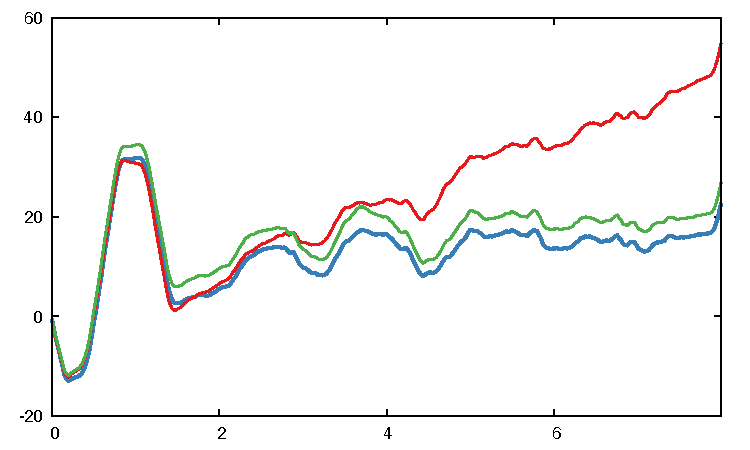
\includegraphics[width=\textwidth]{madg_data/pitch.pdf}
	    \caption{Pitch}
    \label{fig:pitch}
    \end{subfigure}
    \hfill
    \begin{subfigure}[b]{0.327\textwidth}
        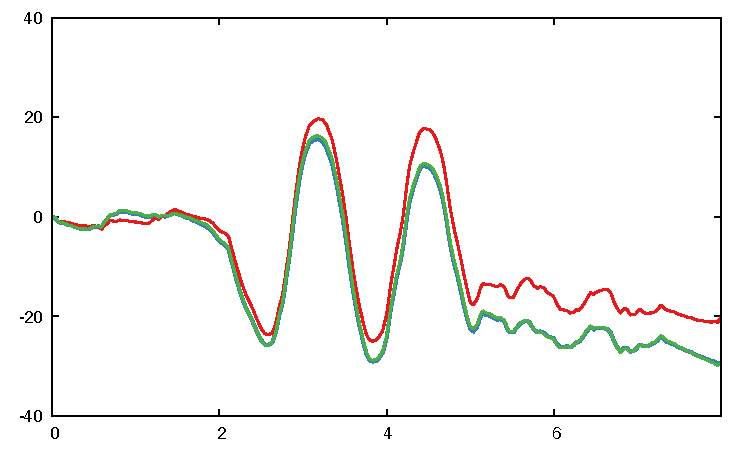
\includegraphics[width=\textwidth]{madg_data/yaw.pdf}
        \caption{Yaw}
        \label{fig:yaw}
    \end{subfigure}
    \hfill
    \begin{subfigure}[b]{0.327\textwidth}
        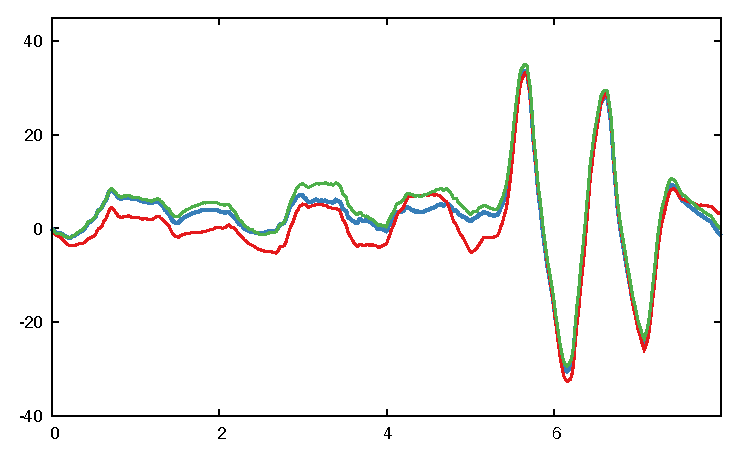
\includegraphics[width=\textwidth]{madg_data/roll.pdf}
        \caption{Roll}
        \label{fig:roll}
    \end{subfigure}
    \hfill
    \caption{Experimental Results: Orientation Estimation of a device oscillating in pitch, yaw, then roll. \textbf{Green} is lifted by InteGreat from \emph{real world} firmware that contains a bug. \textbf{Blue} contains \emph{two} lines: the InteGreat lifted firmware recompiled to correct the gradient calculation, and \emph{a correct} Matlab implementation of Madgwick's algorithm. \textbf{Red}, however, is a compiled firmware using the \emph{faulty} C code included in Madgwick's published report. This version has accumulative error with respect to the earth's magnetic field.}
    \label{fig:madg}
\end{figure*}

\textbf{Quadcopter}
We ran four experiments using different versions of Madgwick's algorithm to showcase InteGreat's ability in detecting bugs and algorithm variants in firmware.
These experiments are depicted in Fig.~\ref{fig:madg}, through a simulation of the quad-copter spinning in three dimensions.
These simulations were performed using Matlab's ``rpy\_9axis'' sensor data.
InteGreat's recovered equations allowed us to detect a missing constant multiply and incorporation of Gyroscopic error values in the implemented version of the firmware, as opposed to the published version, demonstrating the utility of the tool.
While we do not give details on the precise differences due to space constraints, these are present in the original publication and will be discussed within the proposed dissertation.

\textbf{PLC}
The PLC firmware is written for a WAGO 750-881 in the IEC 61131-3 programming language.
The attack in question flipped the proportional gain constant in the first of the firmware's PID calls.
By recovering the continuous equations the firmware image implemented, we were able to \emph{stage} this attack without access to the physical PLC.
However, we also found an obscure scaling was applied in the firmware to the sensor value for the input reactor pressure:

\begin{equation}
    P = 1000(((P_{digital} / 30000) - 0.0046) / 0.9876) + 2000
	\label{eqn:input-conv}
\end{equation}

This was because the actual reactor pressure (which starts at 2800 kPa in the TE simulation), is supplied to the PLC through a \emph{physical wire}, rather than a serial port.
When the Matlab model supplied inputs to the PLC, they were passed through a Digital-to-Analog Converter (DAC).
The original pressure value is converted to a voltage value between 1 and 3, and then this voltage is converted back to a digital value on the physical PLC (30,000) corresponding to 3 volts.

We confirmed this was the case with the ICSREF authors and then proceeded to evaluate our findings on the Matlab environmental model of the chemical plant used in the ICSREF paper.
The scaling equations applied to PLC I/O values in Matlab are \emph{not} the inverse of Eqn.~\ref{eqn:input-conv}.
No scaling was applied to the output in the Firmware's code: the value is simply written to the line.
However, on the Matlab side, a conversion was performed to interpret this signal from the voltage level.

\begin{figure*}
    \centering
    \begin{subfigure}[b]{0.49\textwidth}
        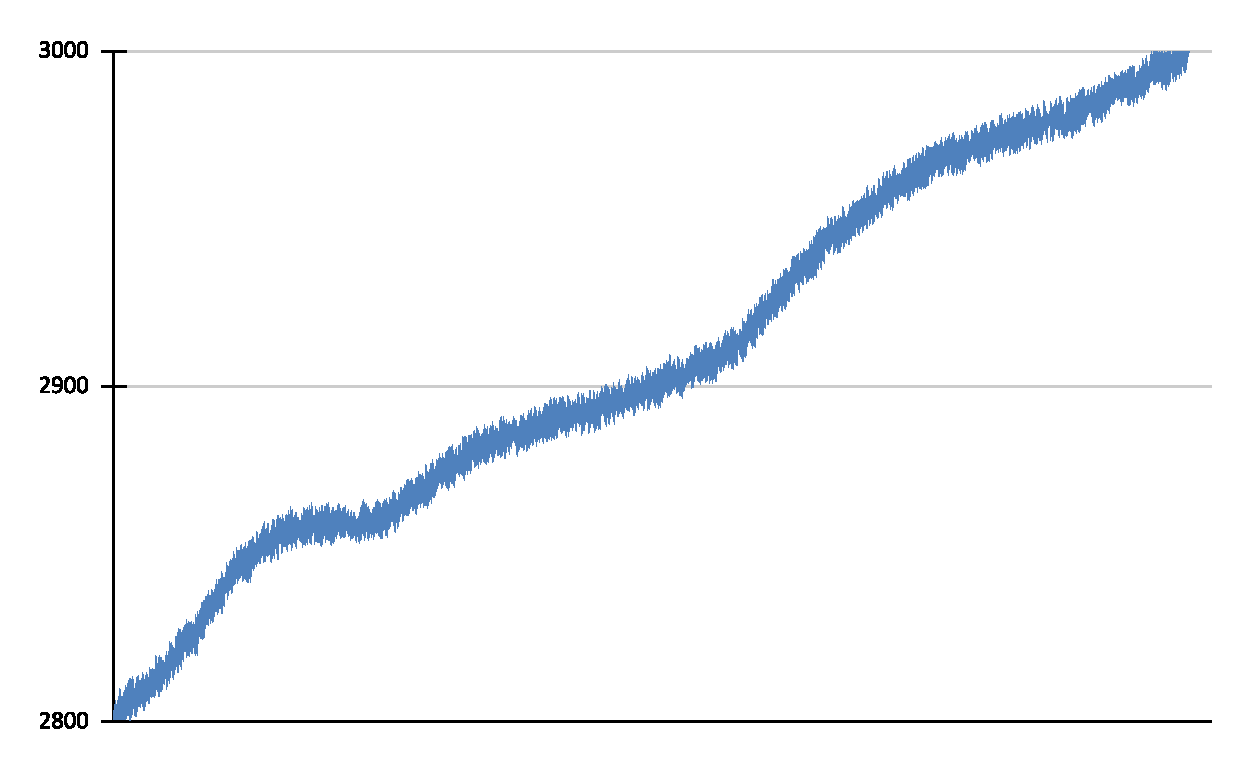
\includegraphics[width=\textwidth]{plc-orig.pdf}
        \caption{Naive Attack Reproduction}
        \label{fig:orig-attack}
    \end{subfigure}
    \hfill
    \begin{subfigure}[b]{0.49\textwidth}
        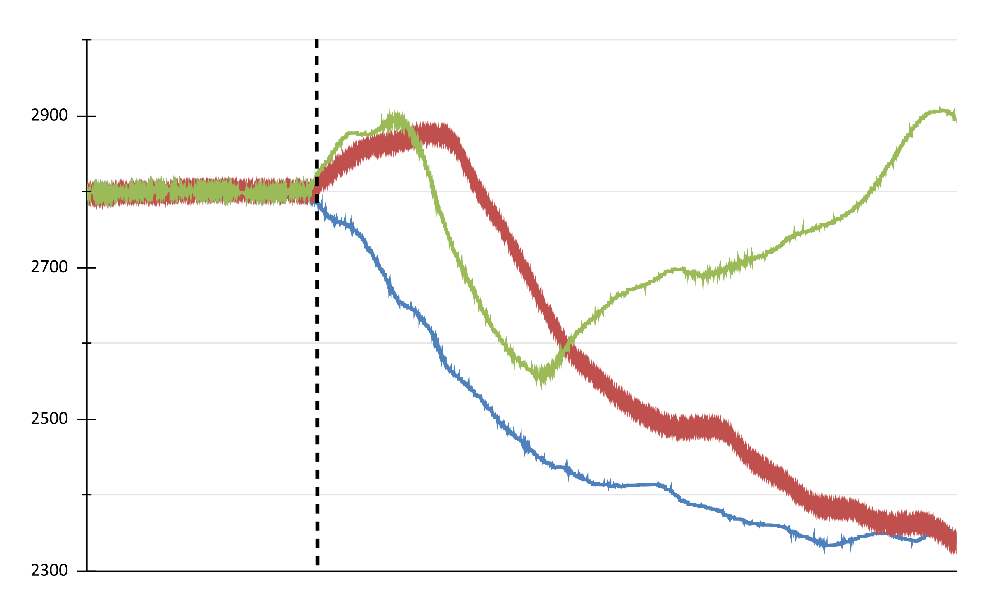
\includegraphics[width=\textwidth]{dashed-plc.pdf}
	    \caption{Voltage Corrected Destabilization}
        \label{fig:noconv-attack}
    \end{subfigure}
    \hfill
	\caption{\textbf{Left}: An attempt to stage the ICSREF attack using the recovered model without taking into account the physical effects of digital-to-analog conversion. \textbf{Right}: Variations of the staged attack with physical effects accounted for. The dashed line is the point at which the attack occurs (the 4 hour mark).}
    \label{fig:plc-eval}
\end{figure*}

Therefore, a naive digital twin of the firmware's implementation, maintaining the original voltage conversions, results in Fig.~\ref{fig:orig-attack} when staging the attack.
This is because, fundamentally, the input and output values to the PLC's equations are affected by the scaling decided by the physical digital-to-analog and analog-to-digital converters.
Code for this scaling does not exist in the firmware.
This proposes the importance of a hybrid approach to modeling in the current domain of firmware rehosting~\cite{jetset,p2im,halucinator}.
While an exact emulation of the firmware's operation is desirable for dynamic analysis and testing (e.g. fuzzing), it is also necessary to verify that the I/O boundaries of the system are consistent with the physical environment or environmental model the emulation is attached to.

Moving forward with this new understanding, we were able to correctly reproduce the destabilizing effects on reactor pressure created by uploading code to the PLC (Fig.~\ref{fig:noconv-attack}).
We corrected for the input value scaling in all cases, but we explore the effects of \emph{adding} semantics for the output scaling created by physical effects.
\textbf{Blue} represents the case where the output voltage is exactly matched to the inputs and outputs of Matlab. \textbf{Red} represents the case where the output voltage is modified to match the physical scaling created by the physical wiring of the PLC. \textbf{Green} represents the case where the attack \emph{did not} occur, and the output voltage scaling is applied to match the dynamics of the physical PLC.
These findings explain the otherwise unexplained ``bump'' in the graph of the original ICSREF paper, and demonstrate how InteGreat can be used to recover an abstract model of a program where no prior model exists.

\subsubsection{Discussion}

Informed by both the Jetset and \emph{Story Beyond the Eye} works, InteGreat adopts an opinionated perspective on the challenges facing binary program analysis.
It attempts to address universal and necessary limitations to abstract interpretation, such as the modeling of microarchitectural semantics and state explosion, by applying the well-worn technique of wrapping these complexities in a layer of abstraction (program slices), and then automates the construction of this abstraction.
While this alleviates the difficulties involved in inferring loop invariants and pointer analysis, InteGreat also has the explicit limitation of requiring users to leave these semantics undefined or provide their own formulae for resolution.

However, the abstraction of complex program semantics is also InteGreat's strength. 
By providing an interface for a more abstract representation the system during symbolic execution, InteGreat is able to rely on additional input for undefined or undecidable cases and extract useful models in cases where no such additional information is required or feasible to provide.
Moreover, by incorporating an object-oriented approach for abstraction specifications, the framework is also able to continually expand its base of knowledge.
The proposed dissertation will detail the trade-offs of abstraction and discuss the conditions under which InteGreat could be applied to the problems presented in Jetset and \emph{Story Beyond the Eye} thoroughly.
